% Tipo de documento y tamaño de letra
\documentclass[letterpaper,10pt,twoside,onecolumn]{article}
\textwidth=15cm
% Preparando para documento en Español.
% Para documento en Inglés no hay que hacer esto.
\usepackage[spanish]{babel}
\usepackage{graphicx}
\selectlanguage{spanish}
\usepackage[utf8]{inputenc}
\begin{document}
 
\title{PRODUCTO 4} 
\author{Ana Magdalena Sotomayor} 

\maketitle 
\section{INTRODUCCION}
Se realizaron códigos para graficar en Maxima, utilizando los comandos de gnuplot para realizar las aproximaciones de Taylor en funciones de senoidales, logarítmicas y exponenciales. 

Fórmula de Taylor

Sea f(x) una función definida en un intervalo que contiene al punto a, con derivada de todos los órdenes.

El polinomio de primer grado p1(x) = f(a) + f ' (a) (x-a) tiene el mismo valor que f(x) en el punto x=a y también, como se comprueba fácilmente, la misma derivada que f(x) en este punto. Su gráfica es una recta tangente a la gráfica de f(x) en el punto a.

Es posible elegir un polinomio de segundo grado,

 $p2(x) = f(a)+f'(a)(x-a)+1/2f''(a)>2...+(1/n!)(f>n(a)(x-a)>n$

tal que en el punto x=a tenga el mismo valor que f(x) y valores también iguales para su primera y segunda derivadas. Su gráfica en el punto a se acercará a la de f(x) más que la anterior. Es natural esperar que si construimos un polinomio que en x=a tenga las mismas n primeras derivadas que f(x) en el mismo punto, este polinomio se aproximará más a f(x) en los puntos x próximos a a. Así obtenemos la siguiente igualdad aproximada, que es la fórmula de Taylor:
$f(x) = f(a) + f'(a)(x-a) + (1/2!)f''(a)(x-a)2+ ...... + (1/n!)f>n(a)(x-a)>n$
El segundo miembro de esta fórmula es un polinomio de grado n en (x-a). Para cada valor de x puede calcularse el valor de este polinomio si se conocen los valores de f(a) y de sus n primeras derivadas.

Para funciones que tienen derivada (n+1)-ésima, el segundo miembro de esta fórmula, como se demuestra fácilmente, difiere del primero en una pequeña cantidad que tiende a cero más rápidamente que (x-a)n. Además, es el único polinomio de grado n que difiere de f(x), para x próximo a a, en un valor que tiende a cero (cuando x tiende a a) más rápidamente que (x-a)n.
Si f(x) es un polinomio algebraico de grado n, entonces la igualdad aproximada anterior es una verdadera igualdad.

Para que sea exacta la igualdad aproximada anterior, debemos añadir al segundo miembro un término más, llamado resto o error:
$f(x) = f(a)+f'(a)(x-a)+(1/2!)+ f''(a)(x-a)>2+ ...... +(1/n!)fn(a)(x-a)n+(1/(n+1)!)+f(n+1)(c)(x-a)(n+1)$

\section{CODIGOS} 
\subsection{Aproximaciones de Taylor para f(x)=sin(x)}
\begin{verbatim}
f(x):= sin(x);

t1(x):=taylor(f(x), x, 0, 1);

t3(x):=taylor(f(x), x, 0, 3);

t5(x):=taylor(f(x), x, 0, 5);

t7(x):=taylor(f(x), x, 0, 7);

fortran(t1(x));

fortran(t3(x));

fortran(t5(x));

fortran(t7(x));

tex(t1(x));

tex(t3(x));

tex(t5(x));

tex(t7(x));

 plot2d ([f(x),t1(x), t3(x), t5(x), t7(x)], [x, -4, 4], [y, -1.5, 1.5],
 [style,[lines,3],[xlabel, "X"], [ylabel, "Y"]],[grid,15,15], 
 [color,red,green,blue,magenta,cyan],  [legend,"y=sin(x)","y=f1(x)",
 "y=f3(x)","y=f5(x)", "y=f7(x)"], [axes, true], [box,false]);

\end{verbatim}

\subsection{Imagen de salida}
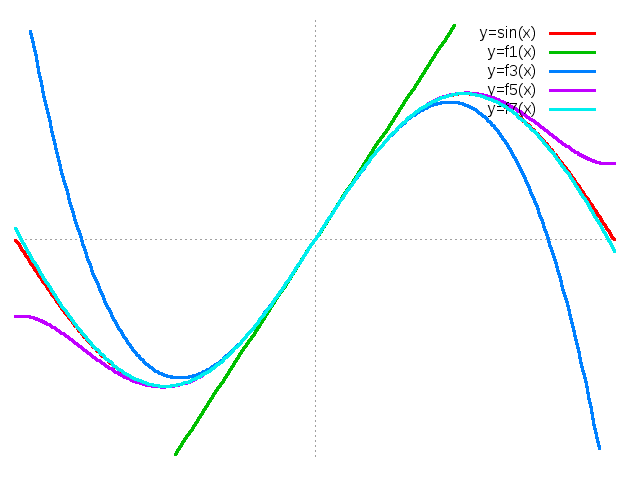
\includegraphics[scale=.55]{Taylor.png}

\subsection{Aproximaciones de Taylor para f(x)=log (1+x)}
\begin{verbatim} f(x):= log (1+x);

t4(x):=taylor(f(x), x, 0, 4);

t7(x):=taylor(f(x), x, 0, 7);

t11(x):=taylor(f(x), x, 0, 11);

t16(x):=taylor(f(x), x, 0, 16);

fortran(t4(x));

fortran(t7(x));

fortran(t11(x));

fortran(t16(x));

tex(t4(x));

tex(t7(x));

tex(t11(x));

tex(t16(x));

plot2d ([t4(x), t7(x), t11(x), t16(x),f(x)], [x, -1.5, 1.5],
 [y, -4, 2], [xlabel, "x"],[ylabel, "f(x)"],[legend, "t4", "t7", 
 "t11", "t16", "f(x)=log 1+X"],[grid, 40,40], [style, [lines, 1.5]], 
 [color,red,green,blue,cyan, magenta]);
\end{verbatim}
\subsection{Imagen de salida}
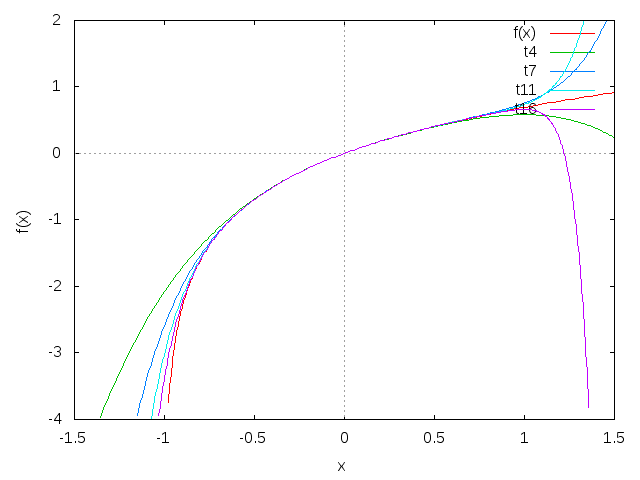
\includegraphics[scale=.55]{Log.png}

\subsection{Aproximaciones de Taylor para f(x)= log(cos(x))}
\begin{verbatim}
f(x):= log(cos(x));

t1(x):=taylor(f(x), x, 0, 1);

t3(x):=taylor(f(x), x, 0, 3);

t5(x):=taylor(f(x), x, 0, 5);

t7(x):=taylor(f(x), x, 0, 7);

fortran(t1(x));

fortran(t3(x));

fortran(t5(x));

fortran(t7(x));

tex(t1(x));

tex(t3(x));

tex(t5(x));

tex(t7(x));

plot2d ([f(x),t1(x), t3(x), t5(x), t7(x)], [x, -%pi/2, %pi/2],
[y, -5, 3], [legend, "f(x)","Taylor grado 1", "Taylor grado 3", 
"Taylor grado 5", "Taylor grado 7"],
[style, [lines, 2]]);
\end{verbatim}
\subsection{Imagen de salida}
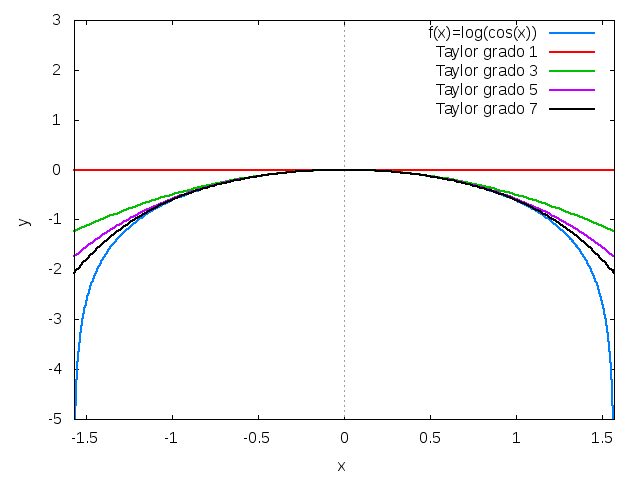
\includegraphics[scale=.55]{LogCos.png}

\subsection{Aproximaciones de Taylor para f(x)= exp(x)/cos(x) }
\begin{verbatim}
f(x):= exp(x)/cos(x);

t2(x):=taylor(f(x), x, 0, 2);

t4(x):=taylor(f(x), x, 0, 4);

t6(x):=taylor(f(x), x, 0, 6);

t8(x):=taylor(f(x), x, 0, 8);

fortran(t2(x));

fortran(t4(x));

fortran(t6(x));

fortran(t8(x));

tex(t2(x));

tex(t4(x));

tex(t6(x));

tex(t8(x));

plot2d ([f(x),t2(x), t4(x), t6(x), t8(x)], [x, -1, 1], 
[legend, "f(x)=exp(x)/cos(x)", "Taylor grado2", "Taylor grado 4", 
"Taylor grado 6","Taylor grado 8"], [style, [lines,2]]);
\end{verbatim}     
\subsection{Imagen de salida}
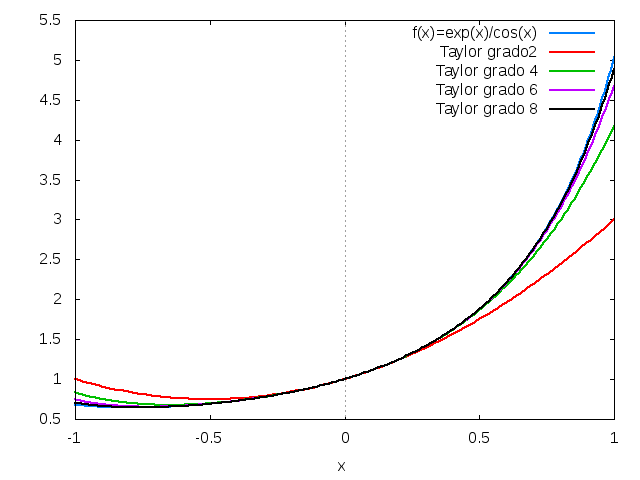
\includegraphics[scale=.55]{ExpCos.png}

\subsection{Aproximaciones de Taylor para f(x)=((1+x)*exp(x))}
\begin{verbatim}
f(x):= ((1+x)*exp(x));

t3(x):=taylor(f(x), x, 0, 3);

t5(x):=taylor(f(x), x, 0, 5);

t7(x):=taylor(f(x), x, 0, 7);

t9(x):=taylor(f(x), x, 0, 9);

fortran(t3(x));

fortran(t5(x));

fortran(t7(x));

fortran(t9(x));

tex(t3(x));

tex(t5(x));

tex(t7(x));

tex(t9(x));

plot2d ([f(x),t3(x), t5(x), t7(x), t9(x)], [x, -5, 5], [y, -2, 2], 
[style, [lines,2]], [legend, "f(x)=((1+x)*exp(x))", "Taylor grado 3", 
"Taylor grado 5", "Taylor grado 7", 
"Taylor grado 9"]);
\end{verbatim}
\subsection{Imagen de salida}

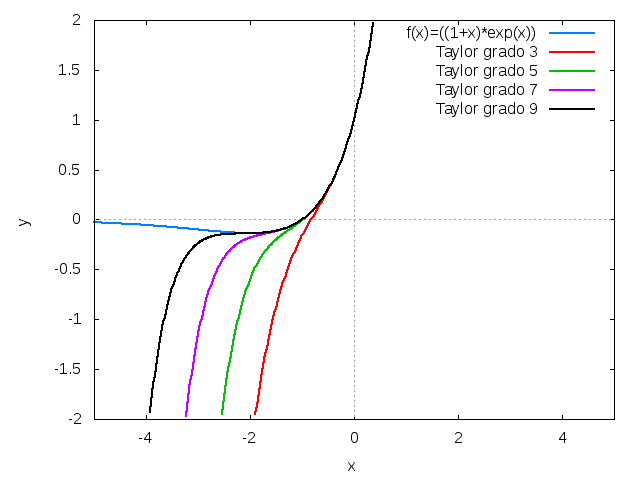
\includegraphics[scale=.55]{linearExp.png}

% Nunca debe faltar esta ultima linea.
\end{document}